\documentclass[11pt]{article}
\usepackage[margin=1.2in]{geometry}
\usepackage{cite}
\usepackage{float}
\usepackage{tikz}
\usepackage{rotating}
\usepackage{lscape}
\usepackage{wrapfig}
\usepackage{pdflscape}
\usepackage{afterpage}

\usepackage{listings}
\lstloadlanguages{[Sharp]C}
\lstnewenvironment{code}
    {\lstset{}%
      \csname lst@SetFirstLabel\endcsname}
    {\csname lst@SaveFirstLabel\endcsname}
    \lstset{
      language=[Sharp]C,
      basicstyle=\small\ttfamily,
      flexiblecolumns=false,
      basewidth={0.5em,0.45em},
      breaklines=true,
      postbreak=\raisebox{0ex}[0ex][0ex]{\ensuremath{\color{red}\hookrightarrow\space}},
    }
\usetikzlibrary{shapes,arrows,positioning}

\tikzstyle{situation} = [rectangle, draw, fill=white!20, 
    text width=10em, text centered, minimum height=4em]
\tikzstyle{action} = [rectangle, draw, fill=white!20, 
    text width=8em, text centered, rounded corners=2em, minimum height=4em]
\tikzstyle{subsumptor} = [circle, draw, fill=white!20,
    text width=2em, text centered]
\tikzstyle{line_n} = [draw, -latex']
\tikzstyle{headless_n} = [draw]
\tikzstyle{anchor_n} = [inner sep=0pt, fill=none, draw=none]

\title{Artificial Intelligence for Games\\
Developing an AI agent for the game of Tanks based on the subsumptive architecture}

\author{Connor Aspinall (13021267) \and George Bell (13025221) \and Denis Torgunov (13011546)}

\date{}

\begin{document}

\newcommand{\includecode}[2][c]{\lstinputlisting[caption=#2, escapechar=, style=custom#1]{#2}<!---->}
\maketitle
\begin{abstract}
  This report details the design and implementation of an AI player for a game of Tanks, based on a subsumptive architecture. We highlight the improvements to our pathfinding module based on what we have learned during our work on the previous coursework, as well as detail our own implementation of subsumptive dispatch. We mention some of the issues we had during development and provide suggestions for future work and improvement.
\end{abstract}
\tableofcontents
\thispagestyle{empty}

\newpage

\section{Introduction}
This report details the implementation of a subsumption-based AI, as developed by the group ``Team \(-i^2\)''. The implementation focuses on an adaptive approach and uses A* for efficient pathfinding and navigation. It is meant to be extendable and the implementation produced, while successful during testing, was envisioned more as a proof of concept, with suggestions on better leveraging the approach proposed given in section~\ref{sec:futureWork}.

Due to the fact that most of the codebase had to be implemented from scratch, as well as time constraints, the resulting AI might not be sufficiently optimised, and therefore unable to utilise CPU time provided in the most efficient manner. Suggestions for further optimisation are also given in section~\ref{sec:futureWork}.

\section{AI Design and Implementation} \label{sec:design}

The AI produced by our group for this coursework focuses on utilising a subsumption architecture, inspired by the work done by one of the group members in the context of intelligent robotics. The subsumptive architecture, as proposed by Brooks, aims to form close connections between sensory inputs and behaviours of an intelligent agent\cite{brooks1}. In the context of an intelligent Tanks player, we can take information gleamed from the state of the map as simulating sensory inputs, and define a series of behaviours (such as running away, exploring, or seeking an enemy) to take in specific situations. This approach lends itself well to group work, as individual components and behaviours can be developed separately, and then combined in arbitrarily complex ways using the subsumption architecture.

The binding of game situations (sensory inputs) to behaviours can be changed dynamically, or assigned at the start. For the purposes of this coursework, we define 2 major ``behaviours profiles'' (as discussed in section~\ref{sec:behaviourProfiles}), a ``Hunter'' and an ``Explorer''. For the discussion of potential for dynamic and adaptive behaviour see section~\ref{sec:futureWork}.
\subsection{Subsumptive Control}

In order to make it possible to implement the subsumptive control system, we have created a class, \verb|SubsumptionDispatch|, which calls the corresponding action when the right ``stimulus'' occurs. For the full source code listing please see section~\ref{sec:subsumptionCode}. In this section we will only highlight the central parts of the implementation.

Firstly, we make use of C\# delegates to allow us to use higher-order methods, passing methods around as values and evoking them when needed. Specifically, we define the following two delegates:

\begin{code}
public delegate bool Situation();
public delegate ICommand Action();
\end{code}

A \verb|Situation| is a predicate that represents a situation in the game, corresponding to sensory input in a traditional subsumption architecture. An \verb|Action| represents a method that returns the next command to execute, corresponding to operating an actuator. It is assumed to take no arguments, relying purely on the internal state of the main class for any information about map composition, current player position, etc.

Having defined those delegates, we can implement a dispatch table as a linked list of tuples:

\begin{code}
private List<Tuple<Situation, Action>> dispatchTable;
\end{code}

We assume that the first element in the list has the highest priority. If its \verb|Situation| arises, we execute the corresponding \verb|Action|. Otherwise, we continue down the list. We assume that at least one of the \verb|Situation|s will occur. In order to ensure that, the final element of the list should be a ``default'' action: simulated using a predicate that is always true.

With those definitions, we can now create the main program loop: the \verb|act()| method:

\begin{code}
public ICommand act()
{
  foreach (Tuple<Situation, Action> behaviour in dispatchTable)
  {
    if (behaviour.Item1())
    {
      return behaviour.Item2();
    }
  }
  return null;
}
\end{code}

As soon as the \verb|Action| with a matching \verb|Situation| is found, we simply execute that action, returning the corresponding command to be executed on this turn.

\subsection{Behaviour Profiles} \label{sec:behaviourProfiles}

We consider two possible behaviour profiles for this AI: the Hunter and the Explorer. The goal of the game is to maximise the score, and the behaviour process aims to do so in the most efficient way. If exploration is more valuable, point-wise, than killing opponents, we can utilise the Explorer profile, which focuses primarily on discovering the map and avoiding confrontation. On the other hand, if the amount of points received for killing an enemy is higher than the amount of points gained (on average) through exploration, we utilise the Hunter profile, which will actively seek to destroy enemy tanks.

Figure~\ref{fig:explorer} outlines the Explorer behaviour profile, and figure~\ref{fig:hunter} outlines Hunter. The Explorer aims to explore as much of the map as possible, while allowing the enemies to fight amongst themselves, only going on the offensive when there is a single enemy left. On the other hand, the Hunter actively seeks to gain points by destroying enemy tanks, and only then explores the remaining parts of the map.

The choice of behaviour profile largely depends on which approach would be more profitable, in terms of points, on a given map. However, since we did not have sufficient data regarding how either profile performs against other AI opponents (see section~\ref{sec:testing} for details), we instead choose to randomise the choice, making it possible for either approach to be chosen when the AI is first loaded in. But, in order to maximise our chances of winning, we bias the randomisation based on score gains for a given terrain.

In particular, as mentioned above, Hunter aims to gain points for killing enemy tanks before other players can do so. But we can only destroy 3 tanks in total, and the gain in points might not be worth the risk. On the other hand, Explorer attempts to avoid confrontation, which might allow the enemy to cut us off from certain portions of the map, diminishing our score.

In the end, we chose to use the following metric: if the average gain for exploring 3/4 of the map is higher than the points gained for killing all 3 tanks, we bias the random profile chooser towards Explorer. Otherwise, the bias is towards Hunter. The ``biased'' profile has a 60\% chance of being picked.

Since the default action implies that there are no enemies left and all of the map has been explored, we simply stay still, as there are no further points to be gained.

\afterpage{
\clearpage
\begin{landscape}
\vspace*{\fill}
\begin{figure}[h]
  \centering
  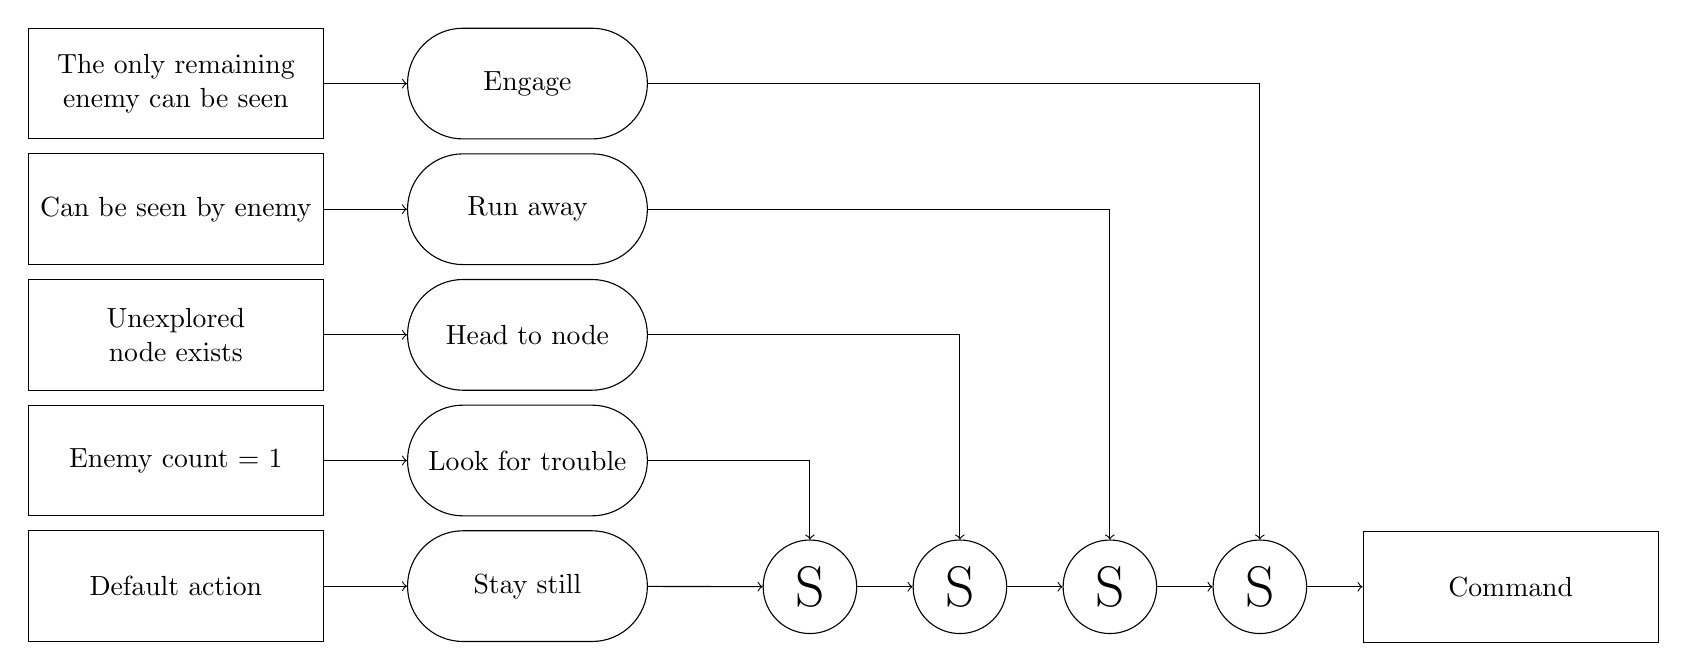
\begin{tikzpicture}[node distance=2cm, auto]
    \node[situation] (finalBoss) {The only remaining enemy can be seen};
    \node[situation,below=0.5em of finalBoss] (enemy) {Can be seen by enemy};
    \node[situation,below=0.5em of enemy] (unexploredNode) {Unexplored node exists};
    \node[situation,below=0.5em of unexploredNode] (singleEnemy) {Enemy count \(=\) 1};
    \node[situation,below=0.5em of singleEnemy] (default) {Default action};

    \node[action,right=3em of finalBoss] (fight) {Engage};
    \node[action,right=3em of enemy] (runAway) {Run away};
    \node[action,right=3em of unexploredNode] (headTo) {Head to node};
    \node[action,right=3em of singleEnemy] (engage) {Look for trouble};
    \node[action,right=3em of default] (stay) {Stay still};

    \node[right=5.5em of engage] (anchorPoint) {};
    
    \node[subsumptor, below=2.5em of anchorPoint] (s1) {\huge S}; 
    \node[subsumptor, right=2em of s1] (s2) {\huge S}; 
    \node[subsumptor, right=2em of s2] (s3) {\huge S}; 
    \node[subsumptor, right=2em of s3] (s4) {\huge S}; 
    
    \node[situation, right=2em of s4] (command) {Command};
    
    \path[draw,->] (default) -- (stay);
    \path[draw,->] (stay) -- (s1);
    \path[draw,->] (s1) -- (s2);
    \path[draw,->] (s2) -- (s3);
    \path[draw,->] (s3) -- (s4);
    \path[draw,->] (s4) -- (command);
    
    \path[draw,->] (finalBoss) -- (fight);
    \path[draw,->] (enemy) -- (runAway);
    \path[draw,->] (unexploredNode) -- (headTo);
    \path[draw,->] (singleEnemy) -- (engage);
    
    \path[draw,->] (engage) -| (s1);
    \path[draw,->] (headTo) -| (s2);
    \path[draw,->] (runAway) -| (s3);
    \path[draw,->] (fight) -| (s4);
  \end{tikzpicture}
  \caption{The Explorer profile}
  \label{fig:explorer}
\end{figure}
\begin{figure}[h]
  \centering
  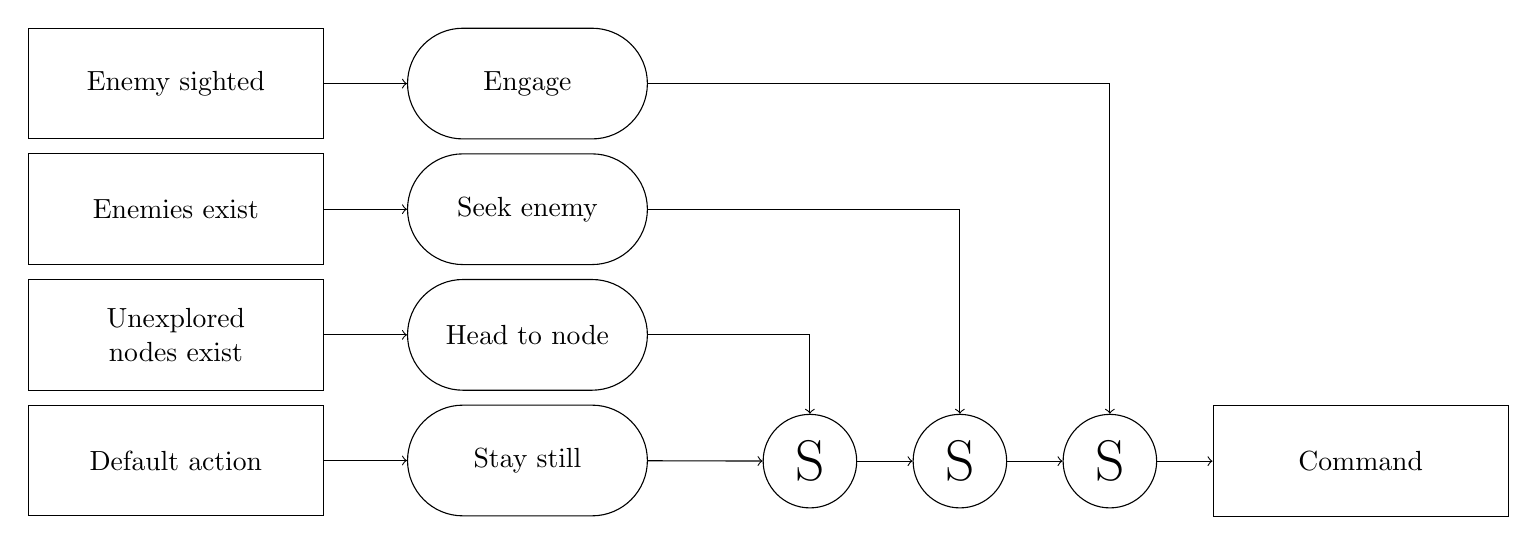
\begin{tikzpicture}[node distance=2cm, auto]
    \node[situation] (enemy) {Enemy sighted};
    \node[situation,below=0.5em of enemy] (unexploredNode) {Enemies exist};
    \node[situation,below=0.5em of unexploredNode] (singleEnemy) {Unexplored nodes exist};
    \node[situation,below=0.5em of singleEnemy] (default) {Default action};

    \node[action,right=3em of enemy] (runAway) {Engage};
    \node[action,right=3em of unexploredNode] (headTo) {Seek enemy};
    \node[action,right=3em of singleEnemy] (engage) {Head to node};
    \node[action,right=3em of default] (stay) {Stay still};

    \node[right=5.5em of engage] (anchorPoint) {};
    
    \node[subsumptor, below=2.5em of anchorPoint] (s1) {\huge S}; 
    \node[subsumptor, right=2em of s1] (s2) {\huge S}; 
    \node[subsumptor, right=2em of s2] (s3) {\huge S}; 
    
    \node[situation, right=2em of s3] (command) {Command};
    
    \path[draw,->] (default) -- (stay);
    \path[draw,->] (stay) -- (s1);
    \path[draw,->] (s1) -- (s2);
    \path[draw,->] (s2) -- (s3);
    \path[draw,->] (s3) -- (command);
    
    \path[draw,->] (enemy) -- (runAway);
    \path[draw,->] (unexploredNode) -- (headTo);
    \path[draw,->] (singleEnemy) -- (engage);
    
    \path[draw,->] (engage) -| (s1);
    \path[draw,->] (headTo) -| (s2);
    \path[draw,->] (runAway) -| (s3);
  \end{tikzpicture}
  \caption{The Hunter profile}
  \label{fig:hunter}
\end{figure}
\vspace*{\fill}
\end{landscape}
}

\subsection{Mapping and Pathfinding}

In order to make it easier to navigate and seek out enemies, we keep track not only of the visible area, but also of the overall map explored so far.  To that end, we have defined a \verb|Cell| enum. We keep and update an array of \verb|Cell|s, filling it with the information about visible parts of the map on each turn. 

We also keep track of the last place we saw enemy tanks, to make it easier to avoid or chase them later. This means that we also have to ``prune'' the map every so often, making sure there is at most one instance of each enemy (the one we saw most recently). For more details, please see section~\ref{sec:aiCode}.

The pathfinding algorithm we use is a refined and improved version of the A* implementation used in our previous coursework submission\cite{theGloriousWe}. We have cleaned up the \verb|GridNode| class, making it more streamlined, smaller and easier to use by removing redundant accessor functions. Since the class is only ever used within the project and no pre-processing of parameters is necessary, and no guarded conditions exist that could be enforced by, we simply made the relevant fields public. The only exception is \verb|GridNode.fCost|, which has been replaced with a getter that simply returns the relevant value, computed based on the other parameters. This reduces the risk of \verb|GridNode.fCost| not being updated properly by mistake.

In addition, we also have completely restructured the main pathfinding logic, in order to remove errors previously present. We have leveraged what we have learned while implementing the first iteration\cite{theGloriousWe} and improved on the main shortcomings.

The most significant changes are as follows:

\begin{itemize}
\item Fixed an issue which caused the \verb|GridNode.fCost| to be set inconsistently while constructing the list of neighbours.
\item Fixed an issue where the path returned is not guaranteed to be the shortest path as some \verb|GridNode|s where skipped unnecessarily.
\item Optimised the implementation by sorting the list to act as a priority queue, potentially reducing CPU time (depending on the native .NET sort implementation).
\item To improve code readability, we use a stack when listing neighbours. We loop through the stack's contents instead of considering each neighbour explicitly when testing whether a coordinate is within the bounds of the board array. Previously, a nested loop was used, but the current approach, in addition to making the code easier to understand, also reduces complexity.
\end{itemize}

For the full listing of the pathfinding code please see section~\ref{sec:pathfindingCode}.

Furthermore, as several actions in our behaviour profiles involve navigating to unexplored parts of the map, we needed a reliable way to determine which unexplored cells we could navigate to. In order to achieve that, we have implemented a function \verb|LocationLocator.UnexploredNode()|, which returns a node at the edge of the currently explored region and not behind a potential wall, if such a node exists. The full code listing is available in section~\ref{sec:locationLocator}, and is based on \cite{denport}.

\subsection{Actions} \label{sec:actions}

The actions that are carried out by the AI are dictated by the Subsumption Dispatch Table, which calls the relevant method in the class \verb|LocationLocator| that, in turn, attempts to find the best location to travel to in the given situation. This is achieved by having several methods, each relevant to one of the potential calls from the Subsumption Dispatch Table, with one being called each turn.

\subsubsection{Retreating}

One of these key actions that can be carried out under the Explorer profile (as can be seen in Figure~\ref{fig:explorer}) is the run away action. This allows the AI to retreat when threatened by an opponent, with the corresponding action being found in the method \verb|LocationLocator.Retreat()|. The full source code is listed in section~\ref{sec:coward}. This method begins by generating a \verb|List| of \verb|GridNode|s found around the player that contain an obstacle that can be hidden behind. This list is initially generated from a 3-by-3 area which is centred on the player, however this will be expanded if no suitable hiding locations are found. Due to the increasing complexity of this algorithm upon expansion\cite{GeorgeComplex}, it is capped at an area of 5-by-5, or an additional \verb|GridNode| in each direction. If, after analysing an area of that size we find no suitable cover, it will default to dodging in a random direction until it moves closer to something it can take cover behind.

Upon finding a valid piece of cover, the AI will check behind it to see if it is a valid location. This is done by comparing the value of the \verb|Cell| to that of \verb|Cell.Empty|. Initially, this is done by looking at any obstacles in the four cardinal directions within GridWorld (Up, Down, Left and Right) and check the side opposite the player. If the these locations are not valid, or if no obstacles exist in these positions, the AI checks the corner \verb|Cell|s. These can potentially have two separate locations where the tank can hide, so both the furthest X and Y locations (relative to the player) must be checked. Again, if there is a valid location to move to and hide at, it will do so, but if there is not then the AI defaults back to the \verb|LocationLocator.RandomDodge()| method.

\verb|LocationLocator.RandomDodge()|, which is used when no hiding places are found close to the player, works to determine where the player should move. The randomness is included so that, if there are multiple moves possible at a given time, it will choose one that cannot be predicted. This behaviour is often seen in video games\cite{GeorgeRandom}, as it can lead to unexpected events occurring for the player, although it is also helpful in this scenario as it enables the AI to be slightly unpredictable, potentially dealing with opponents that implement machine learning.

\subsubsection{Attacking}

The key action from the Hunter profile (Figure~\ref{fig:hunter}) is to find and kill a visible opponent. This action is carried out in the \verb|LocationLocator.Attack()| method, which accepts the following arguments:
\begin{itemize}
\item The \verb|GridSquare| that contains the opponent to attack.
\item A \verb|PlayerWorldState.Facing| that represents the direction the AI is facing.
\item The \verb|Command| to be executed if the opponent cannot be attacked directly.
\end{itemize}

To begin with, the method calculates if it is possible to kill the opponent this turn, proceeding to do so if it is possible. This is achieved by checking if the AI and the opponent share either an X or a Y coordinate. If they do, then the AI calculates whether the tank is currently facing the opponent, before either attacking, or rotating and then attacking the given opponent. If this is not the case, then the \verb|Command| is returned, which is part of a path for the AI to follow towards the opponent. As the tank can only move in four directions, and cannot shoot diagonally, this ensures that the tank will reach a point from which it can attack the given enemy.

\section{Testing and Tuning} \label{sec:testing}

In order to test pathfinding and exploration without the opponent AI destroying us, we have implemented a simple ``Useless'' AI, following the logic described in the lecture notes, that simply stays stationary and avoids attacking. This allowed us to safely navigate around the map and discover the bugs in the exploration part of the code.

In addition, problems arouse due to unexpected errors coming from Visual Studio. Firstly, we got errors trying to load the (standard) \verb|Tuple| class, so we have implemented our own, adhering to the same naming conventions for elements\cite{cSharpTuple}, to make it interoperate with the code already written. In addition, similar errors appeared as the development progressed. Eventually, we have decided to try changing the .NET framework version used by the IDE to 3.5, and while that seemed to resolve the issue, it gave us cryptic warnings that we did not have time to investigate in detail and that might account for some of the bugs.

Due to problems accessing the GridWorld server, all of our testing had to be carried out locally, utilising either the ``Useless'' AI or the stock AI provided. Originally, we were going to tune the performance of the agent by experimenting with different priorities and actions in the behaviour profiles, but as real world performance data was unavailable, it could not be done reliably.

However, a small element of ``learning'' has been noticed during testing. Specifically, if the AI is not reloaded, but the game is simply ``rewound'' to the first turn, we still retain the map layout explored during the previous game.

A few errors have revealed in testing, and subsequently fixed, but overall more refinement is needed before the AI is able to win consistently. In particular, perhaps instead of choosing random cells when exploring or seeking enemies, we need to apply some sort of heuristic that will lead to better overall score.

The only issue we have found is, if multiple AIs are loaded in Explorer mode, they come to a stalemate, as they explore all they can, and then stay still until there is only a single enemy left, which never happens, leading to a tie.

\section{Recommendations for Future Work} \label{sec:futureWork}

As mentioned earlier in section~\ref{sec:design}, it is possible to make this AI better by, instead of providing predefined behaviour profiles, introducing a machine learning aspect by allowing the AI to learn, throughout the game, to associate specific \verb|Situation|s with the best \verb|Action|s, as well as adjusting the priority of each binding accordingly. Genetic programming might be a good fit for such a task. However, because it is impossible to save the information on the GridWorld servers themselves between games, it means that the AI has to learn locally, which severely limits the applicability of this approach within the given setup.

The actions and predicates themselves could be further refined and optimised. As detailed in section~\ref{sec:actions}, the complexity of some actions may be increased, allowing the AI to make more informed decisions. With additional refinement and testing, we could find the right balance between runtime and complexity.  For  attacking the AI carries out, the main addition to make to the predicates would be to calculate whether the player can attack the opponent before they themselves can be attacked, enabling a form of 'fight or flight' mechanism to be implemented.

Our approach to mapping and extracting information from the local map kept is, most likely, the least optimised part of the implementation. In particular, we have to loop through the whole array multiple times on each game loop iteration. Combining the tests performed into a single loop and making predicates simple accessors to the boolean fields holding the information gathered this way should make the code a lot less redundant.

Finally, the pathfinding algorithm, as presented in the code, computes the path anew on each loop iteration. If the target cell has not changed, and there is no change in \verb|Situation|, it should be possible to cache the path initially computed, and simply continue moving as needed, greatly reducing the work done on each game loop iteration.

\subsection{GridWorld Recommendations}
As mentioned above, the main element that we found missing in both this and the previous coursework submission for this module is the ability to retain information between runs on the GridWorld server. If each user was allocated a small amount of storage on the server, or a way to redirect some form of data to a text or binary file that could then be retrieved, it would be possible to view the server as a dynamic learning environment, broadening the applicability of machine learning approaches.

More clarity in representing the game situation and knowledge would make debugging easier. For example, some form of visualisation of a tank firing, as well as a way to simulate the agent's field of view within GridWorld.

\section{Conclusions}
While developing this AI, we have leveraged the skills and knowledge gained both as part of this module, as well as other related subjects. It has provided us with an interesting challenge, and the final intelligent agent produced has a lot of potential. While the submitted version might not be sufficiently tested and optimised, we believe that it could form a strong foundation for an adaptive, intelligent player with emergent intelligent behaviour.

\newpage
% \clearpage
\addcontentsline{toc}{section}{References}
\bibliographystyle{IEEEtran}
\bibliography{IEEEabrv,references}

\newpage
\appendix
\addtocontents{toc}{\protect\setcounter{tocdepth}{1}}
\section{Evidence of Group Work}
Throughout this project's development, Github has been used in order to synchronise our work and communicate issues. Below, we list the final log of git contributions, showing that all the group members have participated. Note that, on average, people with less commits had more code added per commit. The majority of the work on the report has been done as a group.

Merge commits have been omitted from the log for brevity.

\begin{verbatim}
6d5b67b Connor Aspinall      Fill in appendices
4ffe4be Denis Torgunov       Add appendix stubs to the report
5d8fa10 Denis Torgunov       Fix an error that crashes the AI
                             if unexplored node becomes blocked.
21b8de3 Denis Torgunov       Add discussion of biased profile chosing to report
0d09162 Denis Torgunov       Fix seekEnemy() bug with picking random node
4c8cd12 Denis Torgunov       Add a bias in behaviour choosing
aedae05 Denis Torgunov       Make behaviour choise random and fix predicates
248f328 Connor Aspinall      Refactor pathfinding class
e3164ef Denis Torgunov       Refactor code and add random choise of behaviour
f3dded9 George Bell          Refactor of Command use in Attack
d55ee2c George Bell          Refactor and update Attack
4799490 Denis Torgunov       Add behaviour profiles
ef8257d Denis Torgunov       Add the lastEnemySighted() predicate
5f7ad22 Connor Aspinall      Finish seekEnemy()
efa0128 Connor Aspinall      Prototype seekEnemy()
cc02522 Denis Torgunov       Proofread the report
ea81331 George Bell          Update Suggestions
a53e09e George Bell          Finished Attacking subsection
d745b2c George Bell          Added basic explanation to the Attacking.
5f41ed4 Denis Torgunov       Fix exploration
c41bde4 George Bell          Added List to Report.
fa038df George Bell          Refactoring of Attack, Subsections in Report.
e326ca8 George Bell          Report work.
71a3d30 George Bell          New Dodge now correctly considers destoryed tanks cover.
149902c George Bell          Impliemtation of AdvancedDodge.
64c5bef George Bell          Corrected error in SimpleDodge. Started on report.
7b9fa9c Denis Torgunov       Draft up introcution and abstract
7367d06 Denis Torgunov       Fleshed out the pathfinding section
24acfab George Bell          Split Dodge method.
bfc0531 Denis Torgunov       Add notes from discussion
9e19b7c Connor Aspinall      Create prototype for lookForTrouble()
36fc777 Denis Torgunov       Create exploration prototype
c683171 Connor Aspinall      Optimise pathfinding and add testing code
c69b8ff Connor Aspinall      Slim down GridNode
8d6669f Denis Torgunov       Add the section on mapping
a3669cd Denis Torgunov       Prototype goToUnexplored() and UnexploredNode()
ed8ed85 Denis Torgunov       Implement runAway() and engageEnemy()
93b7d95 Denis Torgunov       Reflect the recent changes in the report
e32ea4a Denis Torgunov       Add enemiesExist() and enemySigted() predicates
4e5f290 Denis Torgunov       Reorder methods for redability
c74221e Denis Torgunov       Implement seenByEnemy()
67da775 Connor Aspinall      Update A* Logic
fc6081b Connor Aspinall      Add heuristic, update Gridnode methods
7e320a7 George Bell          Can now move to attack positions.
bfb9eb7 George Bell          No longer crashes when hiding near the edge.
f378b36 Connor Aspinall      Update pathfinding class contructors
8e841eb Denis Torgunov       Outline the seenByEnemy() method
15617bd Denis Torgunov       Add conversion from Cell[,] back to GridSquare[,]
62ae13e George Bell          Basic cardinal attack functionality.
a95cd68 Denis Torgunov       Add the first couple of predicates
50a16f8 George Bell          Advanced hiding mechanics.
dfbe9f1 Denis Torgunov       Fix typo
983b2db George Bell          Basic cardinal direction cover checking
00423f6 Denis Torgunov       Add section on behaviour profiles
965bf83 George Bell          Changed List to GridNode.
a8f44ae Denis Torgunov       Add discussion of SubsumptionDispatch to report
1797f8f George Bell          Added RandomUnkown method.
34d4cd0 George Bell          Added code to regenerate a larger map if it is empty.
b7a68b6 Denis Torgunov       Add overall discussion of design to the report
2e92c30 George Bell          Made list generation a seperate method.
3c858e2 George Bell          Added list of nearby rocks.
cedf709 George Bell          Seperated RandomKnown to a seperate method.
5d27041 Denis Torgunov       Add the report outline
7fc751e George Bell          Added the RandomDodge method.
1ca0096 George Bell          Added return type and base case to Retreat method.
252eca1 George Bell          Added GridSquare for player.
cc36167 George Bell          Basic framework added to LocationLocator.
0e68f3c George Bell          LocationLocator created.
ccdbb64 Denis Torgunov       Add the dispatcher to the main class
defbd1f Denis Torgunov       Create a copy of the Tuple class
3f286e8 Denis Torgunov       Add an (inefficient) way of converting the map
4eb90e4 Connor Aspinall      Add Tiles enum and create function prototypes
610bb88 Connor Aspinall      Add pathfinding classes
65bfde2 Denis Torgunov       Create README.md
45fa195 Denis Torgunov       Add the subsumption dispatcher class
8a333f3 Denis Torgunov       Initial commit
\end{verbatim}

\section{Source code}
Please note that a curved red arrow indicates a linebreak not present in the original code, inserted for readibility.

\subsection{Tuple.cs}
\begin{code}
using System;
using System.Collections.Generic;
using System.Collections;
using System.Linq;
using System.Text;

namespace GridWorld
{
    class Tuple<T1, T2> 
    {
        public T1 Item1;
        public T2 Item2;

        public Tuple(T1 i1, T2 i2) {
            this.Item1 = i1;
            this.Item2 = i2;
        }
   
        public override bool Equals(Object obj) {
            if (obj == null)
            {
                return false;
            }

            Tuple<T1, T2> t2 = obj as Tuple<T1, T2>;
            if ((System.Object)t2 == null)
            {
                return false;
            }
            
            return (this.Item1.Equals(t2.Item1) && this.Item2.Equals(t2.Item2));
        }

        public bool Equals(Tuple<T1, T2> t2)
        {
            return (this.Item1.Equals(t2.Item1) && this.Item2.Equals(t2.Item2));
        }
    }
}
\end{code}
\subsection{GridNode.cs}
\begin{code}
namespace GridWorld
{
    /// <summary>
    /// Stores data about each Node in the game when they are being searched.
    /// </summary>
    class GridNode
    {
        public int x;
        public int y;
        public Cell cell;
        public int hCost;
        public int gCost;
        public bool walkable;
        public GridNode parent;

       public GridNode(int x, int y, Cell cell){

            this.x = x;
            this.y = y;
            this.cell = cell;

            if (cell == Cell.Empty || cell == Cell.Hero)
            {
                walkable = true;
            }
            else
            {
                walkable = false;
            }

        }

        /// <summary>
        /// Returns the F-cost of this GridNode.
        /// </summary>
        /// <returns>The F-cost of this GridNode.</returns>
        public int fCost
        {
            get
            {
                return hCost + gCost;
            }
        }

        public Tuple<int, int> ToTuple()
        {

            return new Tuple<int, int>(x, y);
        }


    }
}

\end{code}
\subsection{MightyPathFinder.cs} \label{sec:pathfindingCode}
\begin{code}
using System;
using System.Collections.Generic;
using System.Linq;
using System.Text;

namespace GridWorld
{
    class MightyPathFinder
    {
        GridNode[,] InternalNodeMap;
        Cell[,] InternalCellMap;
        GridNode Hero;


        /// <summary>
        /// Construct class and initialise internal map representatives.
        /// </summary>
        /// <param name="ICM">Local Cell Map.</param>
        public MightyPathFinder(Cell[,] ICM)
        {
            this.InternalCellMap = ICM;
            ConvertToGridNodeArray(InternalCellMap);
            
        }

       
        /// <summary>
        /// Convert from Cell[,] to GridNode[,] and intialises internal node map.
        /// </summary>
        /// <param name="ICM">Local Cell Map.</param>
        public void ConvertToGridNodeArray(Cell[,] ICM)
        {
            InternalNodeMap = new GridNode[InternalCellMap.GetLength(0),InternalCellMap.GetLength(1)];

            for (int x = 0; x < InternalCellMap.GetLength(0); x++)
            {
                for (int y = 0; y < InternalCellMap.GetLength(1); y++)
                {
                    InternalNodeMap[x, y] = new GridNode(x, y, InternalCellMap[x, y]);

                    if (InternalCellMap[x, y] == Cell.Hero)
                    {
                        Hero = InternalNodeMap[x, y];
                    }
                }
            }
        }

        /// <summary>
        /// Return the horizontal and vertical neighbouring nodes of a given node. 
        /// </summary>
        /// <param name="node"> The current node.</param>
        /// <param name="target">The target node.</param>
        /// <returns>Return a list of all found neigbours(if any).</returns>

        private List<GridNode> GetNeighbours(GridNode node, GridNode target)
        {

            List<GridNode> neighbours = new List<GridNode>();

            Stack<Tuple<int, int>> potentialNeighbours
                    = new Stack<Tuple<int, int>>();

            int x = node.x;
            int y = node.y;

            potentialNeighbours.Push(new Tuple<int, int>(x - 1, y));
            potentialNeighbours.Push(new Tuple<int, int>(x + 1, y));
            potentialNeighbours.Push(new Tuple<int, int>(x, y - 1));
            potentialNeighbours.Push(new Tuple<int, int>(x, y + 1));

            foreach (Tuple<int, int> coor in potentialNeighbours)
            {
                if (IsValidCoordinate(coor))
                {
                    GridNode n = InternalNodeMap[coor.Item1, coor.Item2];
                    if (n.walkable || n.Equals(target))
                    {
                        neighbours.Add(n);
                    }
                }
            }
            return neighbours;
        }
        /// <summary>
        /// Check if an unexplored node is traversable.
        /// </summary>
        /// <param name="node"> Node to be checked.</param>
        /// <returns>'True' if Traversable, 'False' otherwise.</returns>

        private bool reachableUnexplored(GridNode node)
        {
            if (node.cell == Cell.Unexplored)
            {
                Stack<Tuple<int, int>> potentialNeighbours
                   = new Stack<Tuple<int, int>>();

                int x = node.x;
                int y = node.y;

                potentialNeighbours.Push(new Tuple<int, int>(x - 1, y));
                potentialNeighbours.Push(new Tuple<int, int>(x + 1, y));
                potentialNeighbours.Push(new Tuple<int, int>(x, y - 1));
                potentialNeighbours.Push(new Tuple<int, int>(x, y + 1));

                foreach (Tuple<int, int> coor in potentialNeighbours)
                {
                    if (IsValidCoordinate(coor))
                    {
                        GridNode n = InternalNodeMap[coor.Item1, coor.Item2];
                        if (n.walkable)
                        {
                            return true;
                        }
                    }
                }
                return false;
            }
            else
            {
                return false;
            }
        }

        /// <summary>
        /// Check if vector position is contained on the map.
        /// </summary>
        /// <param name="coor">Position.</param>
        /// <returns></returns>

        private bool IsValidCoordinate(Tuple<int, int> coor)
        {
            if (coor.Item1 < 0 || coor.Item2 < 0)
            {
                return false;
            }

            if (coor.Item1 > InternalNodeMap.GetLength(0) - 1
              || coor.Item2 > InternalNodeMap.GetLength(1) - 1)
            {
                return false;
            }

            return true;
        }

        /// <summary>
        /// Return Matthatten heuristic value of cost for moving from one space to an adjacent space.
        /// </summary>
        /// <param name="node">The Current Node</param>
        /// <param name="goal">The Target Node</param>
        /// <returns>Computed cost</returns>
        private int heuristic(GridNode node, GridNode goal)
        {
            int dx = Math.Abs(node.x - goal.x);
            int dy = Math.Abs(node.y - goal.y);

            return dx + dy;
        }
        /// <summary>
        /// Gets the shortest path between two given node positions. 
        /// </summary>
        /// <param name="TupleNode">Target node position</param>
        /// <param name="heroPos"> Starting node position</param>
        /// <returns> List of path nodes</returns>

        public List<GridNode> GetPathToTarget(Tuple<int, int> TupleNode, GridSquare heroPos){

            ConvertToGridNodeArray(InternalCellMap);

            List<GridNode> open = new List<GridNode>();
            List<GridNode> closed = new List<GridNode>();

            GridNode Target = InternalNodeMap[TupleNode.Item1, TupleNode.Item2];
            GridNode heroNode = new GridNode(heroPos.X, heroPos.Y, Cell.Hero);

            open.Add(heroNode);

            while (open.Count > 0)
            {

                open = open.OrderBy(n => n.fCost).ToList(); // treat as priority queue
                GridNode current = open[0];
                open.Remove(current);
                closed.Add(current);

                if (current == Target)
                {
                    List<GridNode> path = new List<GridNode>();

                    while (current != null)
                    {
                        path.Add(current);
                        current = current.parent;
                    }

                    // reverse the path
                    path.Reverse();

                    return path;
                }

                 List<GridNode> neighbours = GetNeighbours(current, Target);
                    foreach (var n in neighbours)
                    {
                        int cost = current.gCost + 1; // assume movement cost is always 1 (even terrain)

                        // .Contains() should be fine, as we're getting all nodes from the array above,
                        // so the node at the same position should have the same address. If this causes
                        // issues, override .Equals()
                        if (open.Contains(n) && cost < n.gCost)
                        {
                            open.Remove(n);
                        }

                        if (!open.Contains(n) && !closed.Contains(n)) {
                            n.gCost = cost;
                            n.hCost = heuristic(n, Target);
                            n.parent = current;
                            open.Add(n);
                        }
                    }
                }
            
            // no path available
            return new List<GridNode>();
        }
    }
}
\end{code}
\subsection{LocationLocator.cs} \label{sec:locationLocator} \label{sec:coward}
\begin{code}
using System;
using System.Collections.Generic;
using System.Linq;
using System.Text;

namespace GridWorld
{
    class LocationLocator
    {

        private Cell[,] localMap;
        private int id;

        private Tuple<int, int> unexplored;

        /// <summary>
        /// Constructs the class.
        /// </summary>
        /// <param name="localMap">Map of the game environment.</param>
        /// <param name="id">The ID of the player.</param>
        public LocationLocator(Cell[,] localMap,  int id)
        {
            this.unexplored = null;
            Update(localMap, id);
        }

        /// <summary>
        /// Updates the localMap
        /// </summary>
        /// <param name="localMap">Map of the game environment.</param>
        /// <param name="id">The ID of the player.</param>
        public void Update(Cell[,] localMap,  int id)
        {
            this.localMap = localMap;
            this.id = id;
        }

        /// <summary>
        /// Gives a location to locate to.
        /// </summary>
        /// <param name="threat">The threat to retreat from.</param>
        /// <param name="hero">The player</param>
        /// <returns>A Tuple with the coordinates of the destination.</returns>
        public Tuple<int, int> Retreat(GridSquare threat, GridSquare hero)
        {
            int mapWidth = localMap.GetLength(0);
            int mapHeigth = localMap.GetLength(1);

            int searchSize = 1;
            List<GridNode> obs = MapObs(searchSize, hero);

            while(obs.Count == 0) 
            {
                if (searchSize < 3)
                {
                    searchSize++;
                    obs = MapObs(searchSize, hero);
                }
                else
                    return RandomDodge(mapWidth, mapHeigth, threat, hero);
            }

            foreach (GridNode gn in obs)
            {
                if (gn.y == hero.Y && SimpleDodgeX(gn.x, gn.y, hero.X).Item1 != -1)
                    return SimpleDodgeX(gn.x, gn.y, hero.X);
                else if (gn.x == hero.X && SimpleDodgeY(gn.y, gn.x, hero.Y).Item1 != -1)
                    return SimpleDodgeY(gn.y, gn.x, hero.Y);
                else if (gn.y > hero.Y)
                {
                    if (gn.y < mapWidth)
                        if (localMap[gn.x, gn.y + 1] == Cell.Empty)
                            return new Tuple<int, int>(gn.x, gn.y + 1);
                        else if (AdvancedDodge(gn, hero).Item1 != -1)
                            return AdvancedDodge(gn, hero);
                }
                else if (gn.y < hero.Y)
                {
                    if (gn.y > 0)
                        if (localMap[gn.x, gn.y - 1] == Cell.Empty)
                            return new Tuple<int, int>(gn.x, gn.y + 1);
                        else if (AdvancedDodge(gn, hero).Item1 != -1)
                            return AdvancedDodge(gn, hero);
                }
            }

            return RandomDodge(mapWidth, mapHeigth, threat, hero);
        }

        /// <summary>
        /// Dodges behind a rock in one of the two cardinal X directions.
        /// </summary>
        /// <param name="gnMain">The axis shared with the Hero.</param>
        /// <param name="gnSec">The axis not shared with the Hero.</param>
        /// <param name="hMain">The Hero coord on the shared axis.</param>
        /// <returns>A Tuple to move to. Will contain -1, -1 if not valid.</returns>
        private Tuple<int, int> SimpleDodgeX(int gnMain, int gnSec, int hMain)
        {
            if (gnMain < hMain && gnMain > 0)
                if (localMap[gnMain - 1, gnSec] == Cell.Empty)
                    return new Tuple<int, int>(gnMain - 1, gnSec);
            if (gnMain > hMain && gnMain < localMap.GetLength(0))
                if (localMap[gnMain + 1, gnSec] == Cell.Empty)
                    return new Tuple<int, int>(gnMain + 1, gnSec);

            return new Tuple<int, int>(-1, -1);
        }

        /// <summary>
        /// Dodges behind a rock in one of the two cardinal Y directions.
        /// </summary>
        /// <param name="gnMain">The axis shared with the Hero.</param>
        /// <param name="gnSec">The axis not shared with the Hero.</param>
        /// <param name="hMain">The Hero coord on the shared axis.</param>
        /// <returns>A Tuple to move to. Will contain -1, -1 if not valid.</returns>
        private Tuple<int, int> SimpleDodgeY(int gnMain, int gnSec, int hMain)
        {
            if (gnMain < hMain && gnMain > 0)
                if (localMap[gnSec, gnMain - 1] == Cell.Empty)
                    return new Tuple<int, int>(gnSec, gnMain - 1);
            if (gnMain > hMain && gnMain < localMap.GetLength(1))
                if (localMap[gnSec, gnMain + 1] == Cell.Empty)
                    return new Tuple<int, int>(gnSec, gnMain + 1);

            return new Tuple<int, int>(-1, -1);
        }

        /// <summary>
        /// Checks if cover either above or below the player can be hidden behind on the X-axis.
        /// </summary>
        /// <param name="gn">The GridNode to hide behind.</param>
        /// <param name="hero">The player location</param>
        /// <returns>A Tuple to move to. Will contain -1, -1 if not valid.</returns>
        private Tuple<int, int> AdvancedDodge(GridNode gn, GridSquare hero)
        {
            if (gn.x > hero.X)
            {
                if (gn.x < localMap.GetLength(0))
                    if (localMap[gn.x + 1, gn.y] == Cell.Empty)
                        return new Tuple<int, int>(gn.x + 1, gn.y);
            }
            else if (gn.x < hero.X)
            {
                if (gn.x > 0)
                    if (localMap[gn.x - 1, gn.y] == Cell.Empty)
                        return new Tuple<int, int>(gn.x - 1, gn.y);
            }

            return new Tuple<int, int>(-1, -1);
        }

        /// <summary>
        /// Maps the obstacles surronding the player.
        /// </summary>
        /// <param name="size">How far away from the player to go.</param>
        /// <param name="hero">The player location</param>
        /// <returns>A list of the nearby obstacles.</returns>
        private List<GridNode> MapObs(int size, GridSquare hero)
        {
            List<GridNode> obs = new List<GridNode>();

            for (int i = hero.X - size; i <= hero.X + size; i++)
            {
                for (int j = hero.Y - size; j <= hero.Y + size; j++)
                {
                    if(IsValidCoordinate(new Tuple<int, int>(i, j)))
                        if (localMap[i, j] == Cell.Rock)
                            obs.Add(new GridNode(i, j, Cell.Rock));
                }
            }
            return obs;
        }

        /// <summary>
        /// Dodges randomly when no hiding place can be found.
        /// </summary>
        /// <param name="w">The width of the board.</param>
        /// <param name="h">The height of the board.</param>
        /// <param name="t">The target to escape from.</param>
        /// <param name="hero">The player location</param>
        /// <returns>A Tuple with the coordinates of the destination.</returns>
        private Tuple<int, int> RandomDodge(int w, int h, GridSquare t, GridSquare hero)
        {
            Random r = new Random();
            
            int xDiff;
            if(hero.X > t.X)
                xDiff = Math.Abs(hero.X - t.X);
            else
                xDiff = Math.Abs(t.X - hero.X);
            
            int yDiff;
            if (hero.Y > t.Y)
                yDiff = Math.Abs(hero.Y - t.Y);
            else
                yDiff = Math.Abs(t.Y - hero.Y);

            if (xDiff < yDiff)          //Closer on the x-axis, dodge vertically
                return Dodge(0, 1, hero);
            else                        //Closer on the y-axis, dodge horizontally
                return Dodge(1, 0, hero);
        }

        /// <summary>
        /// Determines where to dodge.
        /// </summary>
        /// <param name="xAdd">How far to look in the X-direction.</param>
        /// <param name="yAdd">How far to look in the Y-direction.</param>
        /// <param name="hero">The player location.</param>
        /// <returns>A Tuple with the coordinates of the destination.</returns>
        private Tuple<int, int> Dodge(int xAdd, int yAdd, GridSquare hero)
        {
            Random r = new Random();
            if (localMap[hero.X + xAdd, hero.Y + yAdd] != Cell.Rock && localMap[hero.X - xAdd, hero.Y - yAdd] != Cell.Rock && localMap[hero.X + xAdd, hero.Y + yAdd] != Cell.Destroyed && localMap[hero.X - xAdd, hero.Y - yAdd] != Cell.Destroyed)
            {
                if (r.Next(2) == 0)
                    return new Tuple<int, int>(hero.X + xAdd, hero.Y + yAdd);
                else
                    return new Tuple<int, int>(hero.X - xAdd, hero.Y - yAdd);
            }
            if (localMap[hero.X - xAdd, hero.Y - yAdd] != Cell.Rock && localMap[hero.X - xAdd, hero.Y - yAdd] != Cell.Destroyed)
                return new Tuple<int, int>(hero.X - xAdd, hero.Y - yAdd);
            if (localMap[hero.X + xAdd, hero.Y + yAdd] != Cell.Rock && localMap[hero.X + xAdd, hero.Y + yAdd] != Cell.Destroyed)
                return new Tuple<int, int>(hero.X + xAdd, hero.Y + yAdd);

            return RandomKnown(localMap.GetLength(0), localMap.GetLength(1));
        }

        /// <summary>
        /// Makes a decision how to attack.
        /// </summary>
        /// <param name="threat">The enemy to attack</param>
        /// <param name="facing">The direction the player is facing.</param>
        /// <param name="toEnemy">The pathfinder.</param>
        /// <param name="hero">The player location</param>
        /// <returns>The issued command.</returns>
        public Command Attack(GridSquare threat, PlayerWorldState.Facing facing, Command toEnemy, GridSquare hero) 
        {
            if (hero.X == threat.X)
            {
                if (hero.Y > threat.Y)
                    return AttackFacing(facing, PlayerWorldState.Facing.Down, PlayerWorldState.Facing.Right, PlayerWorldState.Facing.Left);
                else if (hero.Y < threat.Y)
                    return AttackFacing(facing, PlayerWorldState.Facing.Up, PlayerWorldState.Facing.Left, PlayerWorldState.Facing.Right);
            }
            else if(hero.Y == threat.Y)
            {
                if (hero.X > threat.X)
                    return AttackFacing(facing, PlayerWorldState.Facing.Left, PlayerWorldState.Facing.Down, PlayerWorldState.Facing.Up);
                else if (hero.X < threat.X)
                    return AttackFacing(facing, PlayerWorldState.Facing.Right, PlayerWorldState.Facing.Up, PlayerWorldState.Facing.Down);
            }

            return toEnemy;
            
        }

        /// <summary>
        /// Attacks if the player is facing an opponent.
        /// </summary>
        /// <param name="facing">The direction the player is facing.</param>
        /// <param name="noRotate">The direction to face when facing the enemy.</param>
        /// <param name="rotateRight">The direction to face when one rotateRight away from the enemy.</param>
        /// <param name="rotateLeft">The direction to face when one rotateLeft away from the enemy.</param>
        /// <returns>A command to execute.</returns>
        private Command AttackFacing(PlayerWorldState.Facing facing, PlayerWorldState.Facing noRotate, PlayerWorldState.Facing rotateRight, PlayerWorldState.Facing rotateLeft)
        {
            if (facing == noRotate)
                return new Command(Command.Move.Down, true);
            else if (facing == rotateRight)
                return new Command(Command.Move.RotateRight, true);
            else if (facing == rotateLeft)
                return new Command(Command.Move.RotateLeft, true);
            else
                return new Command(Command.Move.RotateLeft, false);
        }

        /// <summary>
        /// Gives a random known node to path to.
        /// </summary>
        /// <param name="w">The width of the board.</param>
        /// <param name="h">The height of the board.</param>
        /// <returns>A Tuple with the coordinates of the destination.</returns>
        public Tuple<int, int> RandomKnown(int w, int h)
        {
            Random r = new Random();
            Cell c;
            int x;
            int y;
            do
            {
                x = r.Next(w);
                y = r.Next(h);
                c = localMap[w, h];
            } while (c != Cell.Empty);

            return new Tuple<int, int>(x, y);
        }

        /// <summary>
        /// Find a random cell that we can reach from our current position.
        /// </summary>
        /// <param name="hero">Our current position.</param>
        /// <returns>A reachable cell.</returns>
        public Tuple<int, int> RandomReachable(GridSquare hero)
        {
            List<Tuple<int, int>> reachableCells = ReachableUnexplored(hero);

            for (int x = 0; x < localMap.GetLength(0); x++)
            {
                for (int y = 0; y < localMap.GetLength(1); y++)
                {
                    if ((localMap[x, y] == Cell.Empty || localMap[x, y] == Cell.Hero) // to account for possibly not cleaning Hero right
                        && (x != hero.X && y != hero.Y))
                    {
                        reachableCells.Add(new Tuple<int, int>(x, y));
                    }
                }
            }

            Random r = new Random();
            return reachableCells.ElementAt(r.Next(reachableCells.Count));
        }

        /// <summary>
        /// Refresh the current target unexplored location. Needed in case our path gets blocked off.
        /// </summary>
        public void RefreshUnexplored()
        {
            unexplored = null;
        }

        /// <summary>
        /// Return an unexplored node reachable from our current position.
        /// The node is cached until it ceases being unexplored or is refreshed,
        /// to ensure consistency.
        /// </summary>
        /// <param name="hero">Our current position.</param>
        /// <returns>A reachable unexplored node.</returns>
        public Tuple<int, int> UnexploredNode(GridSquare hero)
        {
            if (unexplored == null)
            {
                SetUnexploredNode(hero); // potential for infinite loop if called with no unexplored nodes remaining
            }

            if (localMap[unexplored.Item1, unexplored.Item2] != Cell.Unexplored)
            {
                SetUnexploredNode(hero);
            }

            return unexplored;
        }

        /// <summary>
        /// Find a random unexplored node that is reachable (i.e. 'pathfindable' from our
        /// current position) and set it as the current "unexplored" target.
        /// </summary>
        /// <param name="hero">The player's position</param>
        private void SetUnexploredNode(GridSquare hero)
        {
            List<Tuple<int, int>> unexplored = ReachableUnexplored(hero);

            if (unexplored.Count == 0)
            {
                this.unexplored = null;
            }

            Random r = new Random();
            this.unexplored = unexplored.ElementAt(r.Next(unexplored.Count));
        }

        /// <summary>
        /// Determine all unexplored nodes reachable from our current position.
        /// </summary>
        /// <param name="hero">Our current position.</param>
        /// <returns>A list of all reachable unexplored nodes.</returns>
        private List<Tuple<int, int>> ReachableUnexplored(GridSquare hero)
        {
            List<Tuple<int, int>> checkedList = new List<Tuple<int, int>>();
            List<Tuple<int, int>> unexplored = new List<Tuple<int, int>>();
            Stack<Tuple<int, int>> toCheck = new Stack<Tuple<int, int>>();

            Tuple<int, int> start = new Tuple<int, int>(hero.X, hero.Y);
            toCheck.Push(start);
            while (toCheck.Count != 0)
            {
                Tuple<int, int> current = toCheck.Pop();

                if (checkedList.Contains(current))
                {
                    continue;
                }

                if (unexplored.Contains(current))
                {
                    continue;
                }

                if (localMap[current.Item1, current.Item2] != Cell.Unexplored)
                {
                    checkedList.Add(current);
                }
                else
                {
                    unexplored.Add(current);
                }

                List<Tuple<int, int>> neightbours = GetNodeNeighbours(current);

                foreach (Tuple<int, int> cell in neightbours)
                {
                    if (!(checkedList.Contains(cell))
                        && !(unexplored.Contains(cell)))
                    {
                        toCheck.Push(cell);
                    }
                }
            }

            return unexplored;
        }

        /// <summary>
        /// Find all the neightbours of a given node, IF that node is not unexplored
        /// or a rock. (This method needs refining!)
        /// </summary>
        /// <param name="node">Coodrinates of a node to start from</param>
        /// <returns>All neighbours of a non-unexplored node</returns>
        private List<Tuple<int, int>> GetNodeNeighbours(Tuple<int, int> node)
        {
            List<Tuple<int, int>> neighbours = new List<Tuple<int, int>>();

           
            if(!potentialWall(node))
            {
                Stack<Tuple<int, int>> potentialNeighbours
                    = new Stack<Tuple<int, int>>();

                int x = node.Item1;
                int y = node.Item2;

                potentialNeighbours.Push(new Tuple<int, int>(x+1, y));
                potentialNeighbours.Push(new Tuple<int, int>(x-1, y));
                potentialNeighbours.Push(new Tuple<int, int>(x, y+1));
                potentialNeighbours.Push(new Tuple<int, int>(x, y-1));

                foreach (Tuple<int, int> coor in potentialNeighbours)
                {
                    if (IsValidCoordinate(coor))
                    {
                        neighbours.Add(coor);
                    }
                }
            }

            return neighbours;
        }

        /// <summary>
        /// Determine whether a block is likely to belong to a "wall" that we can't pathfind around.
        /// </summary>
        /// <param name="coord">Coodrinates of a node to check</param>
        /// <returns>True if coord is a potential element in the middle of a wall, false if it is a passable node or possibly a wall "edge".</returns>
        private bool potentialWall(Tuple<int, int> coord)
        {
            if (passable(coord))
            {
                return false;
            }

            Stack<Tuple<int, int>> leftRight = new Stack<Tuple<int, int>>();
            List<Tuple<int, int>> leftRightValid = new List<Tuple<int, int>>();
            Stack<Tuple<int, int>> upDown = new Stack<Tuple<int, int>>();
            List<Tuple<int, int>> upDownValid = new List<Tuple<int, int>>();

            int x = coord.Item1;
            int y = coord.Item2;

            leftRight.Push(new Tuple<int, int>(x - 1, y));
            leftRight.Push(new Tuple<int, int>(x + 1, y));
            upDown.Push(new Tuple<int, int>(x, y + 1));
            upDown.Push(new Tuple<int, int>(x, y - 1));

            bool result = true;

            foreach (var coor in leftRight)
            {
                if (IsValidCoordinate(coor))
                {
                    result &= nonObsticle(coor);
                }
            }

            if (result)
            {
                return true;
            }

            result = true;

            foreach (Tuple<int, int> coor in upDown)
            {
                if (IsValidCoordinate(coor))
                {
                    result &= nonObsticle(coor);
                }
            }

            return result;
        }

        /// <summary>
        /// Checks if a given node is traversable in terms of pathfinding
        /// </summary>
        /// <param name="coord">Coordinates of a node to check</param>
        /// <returns>True if pathfinding considers the node passable, false otherwise.</returns>
        private bool passable(Tuple<int, int> coord)
        {
            return (localMap[coord.Item1, coord.Item2] == Cell.Empty)
                || (localMap[coord.Item1, coord.Item2] == Cell.Hero);
        }

        /// <summary>
        /// Check if a map is not an obsticle. Since this is used for exploring the map, we consider Unexplored
        /// cells to not be obsticles. Please keep in mind that this should ONLY be used when analyzing a cell
        /// as belonging to a wall or not. A rock with an unexplored cell above it is considered to be at the
        /// "edge", since we don't know if the Unexplored cell is passable or not. However, neighbours of such
        /// cells should not be generated, as that would lead to the whole map being considered reachable.
        /// </summary>
        /// <param name="coord">Coordinates of a node to check</param>
        /// <returns>See method description</returns>
        private bool nonObsticle(Tuple<int, int> coord)
        {
            return passable(coord) || (localMap[coord.Item1, coord.Item2] == Cell.Unexplored);
        }

        /// <summary>
        /// Check if a coordinate is within the bounds of the current map
        /// </summary>
        /// <param name="coor">Coordinate to be checked</param>
        /// <returns>True if coordinate is a valid index into the map array</returns>
        private bool IsValidCoordinate(Tuple<int, int> coor)
        {
            if (coor.Item1 < 0 || coor.Item2 < 0)
            {
                return false;
            }

            if (coor.Item1 > localMap.GetLength(0) - 1
              || coor.Item2 > localMap.GetLength(1) - 1)
            {
                return false;
            }

            return true;
        }
    }
}
\end{code}
\subsection{AI.cs} \label{sec:subsumptionCode} \label{sec:aiCode}
Note that the \verb|SubsumptionDispatch| is an inner class of the main AI class.

\begin{code}
using System;
using System.Collections.Generic;
using System.Linq;
using System.Text;

namespace GridWorld
{
    public enum Cell { Empty, Rock, Hero, Enemy1, Enemy2, Enemy3, Destroyed, Unexplored };
    public class dtorguno : BasePlayer
    {
        /// <summary>
        /// The last known state of the world.
        /// </summary>
        private PlayerWorldState worldState;
        /// <summary>
        /// The local map, keeping track of cells seen and last
        /// known enemy locations.
        /// </summary>
        private Cell[,] localMap;
        /// <summary>
        /// Which player are we?
        /// </summary>
        private int playerNumber;
        /// <summary>
        /// The subsumption dispatcher responsible for
        /// taking the right action in the right situation.
        /// </summary>
        private SubsumptionDispatch dispatcher;

        /// <summary>
        /// The pathfinder module.
        /// </summary>
        private MightyPathFinder pathFinder;
        /// <summary>
        /// The Actions module.
        /// </summary>
        private LocationLocator locationLocator;

        public dtorguno()
            : base()
        {
            this.Name = "A*ship";
            this.localMap = null;
        }

        /// <summary>
        /// Initialise the map on the first turn.
        /// </summary>
        private void initMap() {
            localMap = new Cell[worldState.GridWidthInSquares, 
                                worldState.GridHeightInSquares];

            for (int x = 0; x < worldState.GridWidthInSquares; x++)
            {
                for (int y = 0; y < worldState.GridHeightInSquares; y++)
                {
                    // Simply initialise an empty map. It will be updated
                    // on the first pass
                    localMap[x, y] = Cell.Unexplored;
                }
            }

            this.pathFinder = new MightyPathFinder(localMap);
            this.locationLocator = new LocationLocator(localMap, this.ID);
            this.dispatcher = chooseBehaviour();
        }

        /// <summary>
        /// Randomy choose a behaviour profile. Bias it towards the behaviour that should give us
        /// more points overall.
        /// </summary>
        /// <returns>The subsumption dispatcher corresponding to the chosen profile.</returns>
        private SubsumptionDispatch chooseBehaviour()
        {
            Random r = new Random();
            int choise = r.Next(100);
            int scoreForRock = worldState.ScorePerRockSquareSeen;
            int scoreForEmpty = worldState.ScorePerEmptySquareSeen;
            int scoreForTank = worldState.ScorePerOpposingTankDestroyed;
            double averageExploration = ((double)(scoreForEmpty + scoreForRock)) / 2.0;

            int area = worldState.GridHeightInSquares * worldState.GridWidthInSquares;
            int numberOfEnemies = worldState.PlayerCount - 1;

            // if the average score for exploring 3/4 of the area is bigger than the score
            // for killing all enemies -- bias towards explorer
            double areaScaleFactor = ((double)area) * 3.0 / 4.0;
            SubsumptionDispatch biasTowards, biasAgainst;
            if (areaScaleFactor * averageExploration > numberOfEnemies * scoreForTank)
            {
                biasTowards = explorer();
                biasAgainst = hunter();
            }
            else
            {
                biasTowards = hunter();
                biasAgainst = explorer();
            }

            if (choise < 61)
            {
                return biasTowards;
            }
            else
            {
                return biasAgainst;
            }
        }

        /// <summary>
        /// The main game loop.
        /// </summary>
        /// <param name="igrid">The latest world state.</param>
        /// <returns>A command to execute.</returns>
        public override ICommand GetTurnCommands(IPlayerWorldState igrid)
        {
            worldState = (PlayerWorldState) igrid;

            if (localMap == null)
            {
                initMap();
            }

            updateMap();

            return dispatcher.act();
        }

        // Behavious Profiles

        /// <summary>
        /// The Explorer behaviour profile. Prioratises discovering new squares to confronting enemies,
        /// allowing them to fight amongst themselves instead. Should be used when destroying enemies
        /// is less valuable (in terms of points) than exploring the map.
        /// </summary>
        /// <returns>A subsumption dispatcher corresponding to the Explorer profile.</returns>
        private SubsumptionDispatch explorer()
        {
            SubsumptionDispatch dispatcher = new SubsumptionDispatch();

            dispatcher.add(new Tuple<SubsumptionDispatch.Situation, SubsumptionDispatch.Action>
                (lastEnemySighted, engageEnemy));
            dispatcher.add(new Tuple<SubsumptionDispatch.Situation, SubsumptionDispatch.Action>
                (seenByEnemy, runAway));
            dispatcher.add(new Tuple<SubsumptionDispatch.Situation, SubsumptionDispatch.Action>
                (unexploredExists, goToUnexplored));
            dispatcher.add(new Tuple<SubsumptionDispatch.Situation, SubsumptionDispatch.Action>
                (singleEnemy, seekEnemy));
            dispatcher.add(new Tuple<SubsumptionDispatch.Situation, SubsumptionDispatch.Action>
                (SubsumptionDispatch.defaultAction, stay));
            
            return dispatcher;
        }

        /// <summary>
        /// The Hunter behaviour profile. Prioratises destroying enemies to exploring the map.
        /// Should be used when the gain in points for killing an enemy is larger than point gain
        /// for exploration, in order to stop the enemies from getting those points. Risk if the
        /// reward is high enough.
        /// </summary>
        /// <returns>A subsumption dispatcher corresponding to the Hunter profile.</returns>
        private SubsumptionDispatch hunter()
        {
            SubsumptionDispatch dispatcher = new SubsumptionDispatch();

            dispatcher.add(new Tuple<SubsumptionDispatch.Situation, SubsumptionDispatch.Action>
                (enemySighted, engageEnemy));
            dispatcher.add(new Tuple<SubsumptionDispatch.Situation, SubsumptionDispatch.Action>
                (enemiesExist, seekEnemy));
            dispatcher.add(new Tuple<SubsumptionDispatch.Situation, SubsumptionDispatch.Action>
                (unexploredExists, goToUnexplored));
            dispatcher.add(new Tuple<SubsumptionDispatch.Situation, SubsumptionDispatch.Action>
                (SubsumptionDispatch.defaultAction, stay));

            return dispatcher;
        }

        // Predicates (Situations)

        /// <summary>
        /// Check if there are unexplored cells on the local map.
        /// </summary>
        /// <returns>True if there is at least one unexplored cell, false otherwise.</returns>
        public bool unexploredExists()
        {
            for (int x = 0; x < localMap.GetLength(0); x++)
            {
                for (int y = 0; y < localMap.GetLength(1); y++)
                {
                    if (localMap[x, y] == Cell.Unexplored)
                    {
                        return true;
                    }
                }
            }
            return false;
        }

        /// <summary>
        /// Check if there is only one living enemy.
        /// </summary>
        /// <returns>True if we know exactly one enemy is still alive, false otherwise.</returns>
        public bool singleEnemy()
        {
            return enemyCount() == 1;
        }

        /// <summary>
        /// Check if we are visible to an enemy tank.
        /// </summary>
        /// <returns>True if we can confirm an enemy can see us, false otherwise.</returns>
        public bool seenByEnemy()
        {
            // consider iterating through ALL visible enemies, instead?
            GridSquare enemy = getClosestEnemy();
            if (enemy == null)
            {
                return false;
            }

            GridSquare[,] gs = fromLocalMap();
            int myX = worldState.MyGridSquare.X;
            int myY = worldState.MyGridSquare.Y;
            
            PlayerWorldState.Facing enemyFacing = getFacing(enemy);

            return worldState.CanSee(enemyFacing, enemy.X, enemy.Y, myX, myY, gs);
        }

        /// <summary>
        /// Checks if there is at least one enemy still alive.
        /// </summary>
        /// <returns>True if we know there is more than one living enemy, false otherwise.</returns>
        public bool enemiesExist()
        {
            return enemyCount() > 1;
        }

        /// <summary>
        /// There is (at least one) visible enemy.
        /// </summary>
        /// <returns>True if we can see at least one enemy tank, false otherwise.</returns>
        public bool enemySighted()
        {
            GridSquare closestEnemy = getClosestEnemy();
            if (closestEnemy != null) {
                // the path check is necessary as an enemy who shoots
                // might be visible, but we will not be able to navigate
                // towards it
                List<GridNode> enemyPath = pathFinder.GetPathToTarget(
                    new Tuple<int, int>(closestEnemy.X, closestEnemy.Y), worldState.MyGridSquare);

                return enemyPath.Count > 1;
            }

            return false;
        }

        /// <summary>
        /// We can see (what we know to be) the last enemy tank.
        /// </summary>
        /// <returns>True if the last surviving enemy is visible, false otherwise.</returns>
        public bool lastEnemySighted()
        {
            return enemySighted() && (enemyCount() == 1);
        }

        // Actions

        /// <summary>
        /// Stay still.
        /// </summary>
        /// <returns>The command to execute.</returns>
        public ICommand stay()
        {
            return new Command(Command.Move.Stay, false);
        }

        /// <summary>
        /// Run for cover.
        /// </summary>
        /// <returns>The command to execute.</returns>
        public ICommand runAway()
        {
            GridSquare enemy = getClosestEnemy();
            Tuple<int, int> goHere = locationLocator.Retreat(enemy, worldState.MyGridSquare);
            return urgentMove(goHere);
        }

        /// <summary>
        /// Attempt to attack a visible enemy.
        /// </summary>
        /// <returns>The command to execute.</returns>
        public ICommand engageEnemy()
        {
            GridSquare closestEnemy = getClosestEnemy();

            Command navigateToEnemy = urgentMove(new Tuple<int, int>(closestEnemy.X, closestEnemy.Y));
            return locationLocator.Attack(closestEnemy,
               getFacing(worldState.MyGridSquare), navigateToEnemy, worldState.MyGridSquare);
        }

        /// <summary>
        /// Head in the direction of an unexplored node, using pathfinding to
        /// determine the direction to move in.
        /// </summary>
        /// <returns>The command to execute.</returns>
        public ICommand goToUnexplored()
        {
            Tuple<int, int> dest = locationLocator.UnexploredNode(worldState.MyGridSquare);
            return explorationMove(dest);
        }

        /// <summary>
        /// Move to the last known enemy location, or to a random reachable (explored or not)
        /// cell, hoping to find an enemy.
        /// </summary>
        /// <returns>The command to execute.</returns>
        public ICommand seekEnemy()
        {
            List<Tuple<int, int>> Enemies = new List<Tuple<int, int>>();

            for (int x = 0; x < localMap.GetLength(0); x++)
            {
                for (int y = 0; y < localMap.GetLength(1); y++)
                {

                    if (Enemies.Count == enemyCount())
                    {
                        break;
                    }

                    // if the cell contaions is an enemy tank place in enemy list
                    if (localMap[x, y] == Cell.Enemy1 || localMap[x, y] == Cell.Enemy2 || localMap[x, y] == Cell.Enemy3)
                    {
                        Enemies.Add(new Tuple<int, int>(x, y));
                    }
                }
            }
            
            int cost = int.MaxValue;
            Tuple<int, int> ApproxClosest = null;
            Tuple<int, int> HeroTank = new Tuple<int, int>(worldState.MyGridSquare.X, worldState.MyGridSquare.Y);

            foreach (var tank in Enemies)
            {
                if (squaredDistance(tank, HeroTank) < cost)
                {
                    List<GridNode> path = pathFinder.GetPathToTarget(tank,
                        worldState.MyGridSquare);
                    if (path.Count > 1)
                    {
                        ApproxClosest = tank;
                        cost = squaredDistance(tank, HeroTank);
                    }
                }
            }
            
            if (ApproxClosest != null)
            {
                return explorationMove(ApproxClosest);
            }

            // no known enemy locations, move to a random reachable cell
            Tuple<int, int> potentialCell = locationLocator.RandomReachable(worldState.MyGridSquare);
            List<GridNode> path2 = pathFinder.GetPathToTarget(potentialCell,
                        worldState.MyGridSquare);
            while (!(path2.Count > 1))
            {
                potentialCell = locationLocator.RandomReachable(worldState.MyGridSquare);
                path2 = pathFinder.GetPathToTarget(potentialCell,
                        worldState.MyGridSquare);
            }

            return explorationMove(potentialCell);
        }

        

        // Helper methods

        /// <summary>
        /// Update the internal map as necessary, based on the information from 
        /// currently visible cells.
        /// </summary>
        public void updateMap()
        {
            GridSquare hero = worldState.MyGridSquare;
            playerNumber = hero.Player;
            List<GridSquare> visibleMap = worldState.MyVisibleSquares;

            localMap[hero.X, hero.Y] = Cell.Hero;

            Tuple<int, int> e1 = new Tuple<int, int>(-1, -1);
            Tuple<int, int> e2 = new Tuple<int, int>(-1, -1);
            Tuple<int, int> e3 = new Tuple<int, int>(-1, -1);
            
            foreach (GridSquare square in visibleMap)
            {
                if (hero.X == square.X && hero.Y == square.Y)
                {
                    // already set
                    continue;
                }

               localMap[square.X, square.Y] = convertToCell(square);

               if (localMap[square.X, square.Y] == Cell.Enemy1)
               {
                   e1 = new Tuple<int, int>(square.X, square.Y);
               }
               else if (localMap[square.X, square.Y] == Cell.Enemy2)
               {
                   e2 = new Tuple<int, int>(square.X, square.Y);
               }
               else if (localMap[square.X, square.Y] == Cell.Enemy3)
               {
                   e3 = new Tuple<int, int>(square.X, square.Y);
               }
            }

            cleanTanks(e1, e2, e3);
         }

        /// <summary>
        /// A movement command that tries to maximise the area explored
        /// by turning in the direction of movement before executing a
        /// move.
        /// </summary>
        /// <param name="destination">A location we're trying to move towards.</param>
        /// <returns>The command to execute.</returns>
        private Command explorationMove(Tuple<int, int> destination)
        {
            Command.Move expectedBearing = directionToMove(destination);
            PlayerWorldState.Facing bearing = worldState.MyFacing;

            if (equivalentBearing(bearing, expectedBearing))
            {
                return moveInDirection(destination);
            }
            else
            {
                return turnToFace(destination);
            }
        }

        // move without turning

        /// <summary>
        /// A movement command mainly used for dodging, that forgoes
        /// turning to get out of the enemy's line of fire quickly.
        /// </summary>
        /// <param name="destination">A location we're moving towards.</param>
        /// <returns>The command to execute.</returns>
        private Command urgentMove(Tuple<int, int> destination)
        {
            return moveInDirection(destination);
        }

        /// <summary>
        /// Move in the direction of a given coordinate.
        /// </summary>
        /// <param name="destination">Coordinate to move towards.</param>
        /// <returns>The command to execute.</returns>
        private Command moveInDirection(Tuple<int, int> destination)
        {
            return new Command(directionToMove(destination), false);
        }

        /// <summary>
        /// Turn to face a specific node. Note that if the note is behind
        /// us, the command will need to be executed twice, as no 180 turn
        /// is available.
        /// </summary>
        /// <param name="destination">Coordinate to face.</param>
        /// <returns>The command to execute.</returns>
        private Command turnToFace(Tuple<int, int> destination)
        {
            return new Command(directionToTurn(destination), false);
        }

        /// <summary>
        /// Check whether we are facing the direction we're about to move
        /// towards.
        /// </summary>
        /// <param name="bearing">The direction we're facing.</param>
        /// <param name="expectedBearing">The direction we're about to move in.</param>
        /// <returns>True if the two coincide, false otherwise.</returns>
        private bool equivalentBearing(PlayerWorldState.Facing bearing,
                                        Command.Move expectedBearing)
        {
            return (bearing == PlayerWorldState.Facing.Down 
                    && expectedBearing == Command.Move.Down)
                || (bearing == PlayerWorldState.Facing.Up 
                    && expectedBearing == Command.Move.Up)
                || (bearing == PlayerWorldState.Facing.Left 
                    && expectedBearing == Command.Move.Left)
                || (bearing == PlayerWorldState.Facing.Right 
                    && expectedBearing == Command.Move.Right);
        }

        /// <summary>
        /// The direction we need to move in in order to get closer to a given
        /// coordinate.
        /// </summary>
        /// <param name="destination">The coordinates of the node to move towards.</param>
        /// <returns>The direction of movement.</returns>
        private Command.Move directionToMove(Tuple<int, int> destination)
        {
            List<GridNode> path = pathFinder.GetPathToTarget(destination, worldState.MyGridSquare);
            GridSquare hero = worldState.MyGridSquare;

            // sometimes the enemy comes into the only possible path and we cannot move
            // in those cases, change destination

            if (path.Count < 1)
            {
                //return Command.Move.Stay;
                locationLocator.RefreshUnexplored();
                Tuple<int, int> newDestination = locationLocator.UnexploredNode(hero);
                path = pathFinder.GetPathToTarget(newDestination, worldState.MyGridSquare);
            }

            GridNode nextMove = path.ElementAt(1);
            if (nextMove.x > hero.X)
            {
                return Command.Move.Right;
            }
            else if (nextMove.x < hero.X)
            {
                return Command.Move.Left;
            }
            else if (nextMove.y > hero.Y)
            {
                return Command.Move.Up;
            }
            else
            {
                return Command.Move.Down;
            }
        }

        /// <summary>
        /// The direction we need to turn in in order to face a given coordinate.
        /// </summary>
        /// <param name="destination">The coordinates of the node to face.</param>
        /// <returns>The direction to turn in.</returns>
        private Command.Move directionToTurn(Tuple<int, int> destination)
        {
            Command.Move bearing = directionToMove(destination);

            if (bearing == Command.Move.Right)
            {
                return Command.Move.RotateRight;
            }
            else if (bearing == Command.Move.Left)
            {
                return Command.Move.RotateLeft;
            }
            else
            { // will need to turn twice
                return Command.Move.RotateLeft;
            }
        }

        /// <summary>
        /// Clean duplicate enemies off the map, if the enemy has been sighted again. Also make sure there is only one hero
        /// tank present.
        /// </summary>
        /// <param name="e1">The current known coordinates of the first enemy (or (-1, -1) if not see this turn).</param>
        /// <param name="e2">The current known coordinates of the second enemy (or (-1, -1) if not see this turn).</param>
        /// <param name="e3">The current known coordinates of the third enemy (or (-1, -1) if not see this turn).</param>
        private void cleanTanks(Tuple<int, int> e1, Tuple<int, int> e2, Tuple<int, int> e3)
        {
            for (int x = 0; x < worldState.GridWidthInSquares; x++)
            {
                for (int y = 0; y < worldState.GridHeightInSquares; y++)
                {
                    if (e1.Item1 != -1)
                    {
                        if (localMap[x, y] == Cell.Enemy1
                            && e1.Item1 != x && e1.Item2 != y)
                        {
                            localMap[x, y] = Cell.Empty;
                        }
                    }

                    if (e2.Item1 != -1)
                    {
                        if (localMap[x, y] == Cell.Enemy2
                            && e2.Item1 != x && e2.Item2 != y)
                        {
                            localMap[x, y] = Cell.Empty;
                        }
                    }

                    if (e3.Item1 != -1)
                    {
                        if (localMap[x, y] == Cell.Enemy3
                            && e3.Item1 != x && e3.Item2 != y)
                        {
                            localMap[x, y] = Cell.Empty;
                        }
                    }

                    if (localMap[x, y] == Cell.Hero)
                    {
                        if (worldState.MyGridSquare.X != x || worldState.MyGridSquare.Y != y)
                        {
                            localMap[x, y] = Cell.Empty;
                        }
                    }

                }
            }
        }

        /// <summary>
        /// Convert a grid square to a corresponding cell.
        /// </summary>
        /// <param name="s">The grid square to convert.</param>
        /// <returns>The equivalent cell.</returns>
        private Cell convertToCell(GridSquare s)
        {
            switch (s.Contents)
            {
                case GridSquare.ContentType.Empty:
                    return Cell.Empty;
                case GridSquare.ContentType.Rock:
                    return Cell.Rock;
                case GridSquare.ContentType.DestroyedTank:
                    return Cell.Destroyed;
                case GridSquare.ContentType.TankDown:
                case GridSquare.ContentType.TankLeft:
                case GridSquare.ContentType.TankRight:
                case GridSquare.ContentType.TankUp:
                    return resolveTank(s);
                default:
                    return Cell.Unexplored;
            }
        }

        /// <summary>
        /// Undo the transformation done by convertToCell
        /// </summary>
        /// <param name="c">The cell to convert.</param>
        /// <param name="x">Its x coordinate.</param>
        /// <param name="y">Its y coordinate.</param>
        /// <returns>The equivalent GridSquare.</returns>
        private GridSquare convertFromCell(Cell c, int x, int y)
        {
            switch (c)
            {
                case Cell.Empty:
                    return new GridSquare(x, y, GridSquare.ContentType.Empty);
                case Cell.Destroyed:
                    return new GridSquare(x, y, GridSquare.ContentType.DestroyedTank);
                case Cell.Rock:
                    return new GridSquare(x, y, GridSquare.ContentType.Rock);
                case Cell.Hero:
                case Cell.Enemy1:
                case Cell.Enemy2:
                case Cell.Enemy3:
                    return unresolveTank(x, y);
                case Cell.Unexplored:
                    return new GridSquare(x, y); // assume "empty"
                default:
                    return null;
            }
        }

        /// <summary>
        /// Convert a GridSquare representing an enemy tank to
        /// the right Enemy Cell.
        /// </summary>
        /// <param name="s">A GridSquare representing an enemy.</param>
        /// <returns>The Cell corresponding to the Enemy (does not take bearing into account, but differs per player ID)</returns>
        private Cell resolveTank(GridSquare s)
        {
            // assuming it's not us, or we wouldn't be here
            if (playerNumber == 1 || playerNumber == 4)
            {
                if (s.Player == 2)
                {
                    return Cell.Enemy1;
                }
                else if (s.Player == 3)
                {
                    return Cell.Enemy2;
                }
                else
                {
                    return Cell.Enemy3;
                }
            } else if (playerNumber == 2)
            {
                if (s.Player == 1)
                {
                    return Cell.Enemy1;
                }
                else if (s.Player == 3)
                {
                    return Cell.Enemy2;
                }
                else
                {
                    return Cell.Enemy3;
                }
            } else  // (playerNumber == 3)
            {
                if (s.Player == 2)
                {
                    return Cell.Enemy1;
                }
                else if (s.Player == 1)
                {
                    return Cell.Enemy2;
                }
                else
                {
                    return Cell.Enemy3;
                }
            }            
        }

        /// <summary>
        /// Undo the transformation done by resolveTank. Only works on tanks we can see
        /// (or we wouldn't know the direction they are facing).
        /// </summary>
        /// <param name="x">The x coordinate of the tank.</param>
        /// <param name="y">The y coordinate of the tank.</param>
        /// <returns>The equivalent GridSquare.</returns>
        private GridSquare unresolveTank(int x, int y)
        {
            List<GridSquare> visible = worldState.MyVisibleSquares;
            foreach (GridSquare square in visible)
            {
                if (square.X == x && square.Y == y)
                {
                    return square;
                }
            }

            // tanks only matter when we can see them
            return new GridSquare(x, y, GridSquare.ContentType.Empty);
        }

        /// <summary>
        /// Find the closest enemy tank that we can see.
        /// </summary>
        /// <returns>The closest visible enemy tank, or null if no enemy tanks are visible.</returns>
        private GridSquare getClosestEnemy()
        {
            List<GridSquare> visible = worldState.MyVisibleSquares;
            GridSquare enemySquare = null;
            Tuple<int, int> enemy = null;
            GridSquare hero = worldState.MyGridSquare;
            foreach (GridSquare square in visible)
            {
                if (!isTank(square))
                {
                    continue;
                }

                if (square.X == hero.X && square.Y == hero.Y)
                {
                    continue;
                }

                // this is a tank which is not the hero
                if (enemy == null)
                {
                    // first tank found
                    enemy = new Tuple<int, int>(square.X, square.Y);
                    enemySquare = square;
                }
                else
                {
                    // another tank exists, keep the closes one
                    Tuple<int, int> enemy2 = new Tuple<int, int>(square.X, square.Y);
                    Tuple<int, int> h = new Tuple<int, int>(hero.X, hero.Y);
                    enemy = closest(h, enemy, enemy2);
                    if (enemy.Equals(enemy2))
                    {
                        enemySquare = square;
                    }
                }
            }
            return enemySquare;
        }

        /// <summary>
        /// Determine which of the two coordinate pairs is closest to a given point.
        /// </summary>
        /// <param name="h">Reference point.</param>
        /// <param name="p">First coordinate pair.</param>
        /// <param name="q">Second coordinate pair.</param>
        /// <returns>p or q, depending on which is closest to h.</returns>
        private Tuple<int, int> closest(Tuple<int, int> h, Tuple<int, int> p, Tuple<int, int> q)
        {
            // Use squared Euclidean distance, as it is good enough and quicker to compute
            if (squaredDistance(h, p) >= squaredDistance(h, q))
            {
                return p;
            }
            else
            {
                return q;
            }
        }

        /// <summary>
        /// Compute the squared Euclidean distance between two points.
        /// </summary>
        /// <param name="p">The first point.</param>
        /// <param name="q">The second point.</param>
        /// <returns>The squared Euclidean distance between p and q.</returns>
        private int squaredDistance(Tuple<int, int> p, Tuple<int, int> q)
        {
            int deltaX = q.Item1 - p.Item1;
            int deltaY = q.Item2 - p.Item2;
            return deltaX * deltaX + deltaY * deltaY;
        }

        /// <summary>
        /// Check whether a GridSquare is occupied by a tank.
        /// </summary>
        /// <param name="s">The GridSquare to consider.</param>
        /// <returns>True if s is a tank, false otherwise.</returns>
        private bool isTank(GridSquare s)
        {
            return (s.Contents == GridSquare.ContentType.TankDown)
                || (s.Contents == GridSquare.ContentType.TankUp)
                || (s.Contents == GridSquare.ContentType.TankLeft)
                || (s.Contents == GridSquare.ContentType.TankRight);
        }

        /// <summary>
        /// Undo the conversion to localMap done by updateMap(). Note that there is some loss
        /// of information: namely, the tanks that are not visible are not taken into account.
        /// </summary>
        /// <returns>A (semi)equivalent GridSquare map, corresponding to our internal map.</returns>
        private GridSquare[,] fromLocalMap()
        {
            GridSquare[,] gs = new GridSquare[localMap.GetLength(0), localMap.GetLength(1)];
            for (int x = 0; x < localMap.GetLength(0); x++)
            {
                for (int y = 0; y < localMap.GetLength(1); y++)
                {
                    gs[x, y] = convertFromCell(localMap[x, y], x, y);
                }
            }

            return gs;
        }

        /// <summary>
        /// Determine the facing of a tank.
        /// </summary>
        /// <param name="tank">A GridSquare containing a tank.</param>
        /// <returns>The direction that tank is facing.</returns>
        private PlayerWorldState.Facing getFacing(GridSquare tank)
        {
            switch (tank.Contents)
            {
                case GridSquare.ContentType.TankDown:
                    return PlayerWorldState.Facing.Down;
                case GridSquare.ContentType.TankLeft:
                    return PlayerWorldState.Facing.Left;
                case GridSquare.ContentType.TankRight:
                    return PlayerWorldState.Facing.Right;
                case GridSquare.ContentType.TankUp:
                    return PlayerWorldState.Facing.Up;
                default:
                    // shouldn't happen
                    return PlayerWorldState.Facing.Down;
            }
        }

        /// <summary>
        /// The amount of known enemies. Only destroyed tanks that have been observed
        /// are subtracted from this count.
        /// </summary>
        /// <returns>The (estimated) number of enemies alive, based on map data.</returns>
        private int enemyCount()
        {
            int totalEnemyCount = worldState.PlayerCount - 1;
            int aliveEnemyCount = totalEnemyCount;
            for (int x = 0; x < localMap.GetLength(0); x++)
            {
                for (int y = 0; y < localMap.GetLength(1); y++)
                {
                    if (localMap[x, y] == Cell.Destroyed)
                    {
                        // subtract the enemies we know are destroyed
                        aliveEnemyCount--;
                    }
                }
            }

            return aliveEnemyCount;
        }

        class SubsumptionDispatch
        {
            public delegate bool Situation();
            public delegate ICommand Action();

            // the FIRST action in the table has HIGHEST priority
            
            /// <summary>
            /// A dispatch table mapping Situations to Actions
            /// </summary>
            private List<Tuple<Situation, Action>> dispatchTable;

            
            public SubsumptionDispatch()
            {
                this.dispatchTable = new List<Tuple<Situation, Action>>();
            }

            public SubsumptionDispatch(List<Tuple<Situation, Action>> dispatchTable)
            {
                this.dispatchTable = dispatchTable;
            }

            /// <summary>
            /// Add a new entry to the dispatch table, with lowest priority
            /// </summary>
            /// <param name=''entry''>An entry to add</param>
            public void add(Tuple<Situation, Action> entry)
            {
                dispatchTable.Add(entry);
            }

            /// <summary>
            /// A way to represent a default action Situation.
            /// </summary>
            /// <returns>Always true</returns>
            public static bool defaultAction()
            {
                return true;
            }

            /// <summary>
            /// Pick the appropriate action from the dispatch table and return its command
            /// </summary>
            /// <returns>The command to execute, given the current situation</returns>
            public ICommand act()
            {
                foreach (Tuple<Situation, Action> behaviour in dispatchTable)
                {
                    if (behaviour.Item1())
                    {
                        return behaviour.Item2();
                    }
                }

                // isn't reachable if the default action is given
                return null;
            }
        }
    }
}
\end{code}

\end{document}
